\chapter{Initial and final GANTT Chart}
\centerline{\rule{149mm}{.02in}}
\vspace{2cm}

Below are the initial and final GANTT Charts for this project. As you will see, much of the structure of the project remained the same, such as the general flow from research, to implementation, to write-up. One considerable difference in this respect is that each part took much longer than anticipated, meaning there was a little more overlap in tasks, and the project was finished slightly later than expected. \\ 

You will also notice that there is a good deal more planning work in the final schedule, in particular around half way through the project. This has been explained in the Evaluation of this chapter, and comes from the general need for a re-think of the meaning of an 'Evaluation' and the real aims and objectives of the project. \\

Other than these points, the GANTT charts remained very similar, showing that the work in this project was well planned, organised and executed. 


\begin{sidewaysfigure}
\centering
\fbox{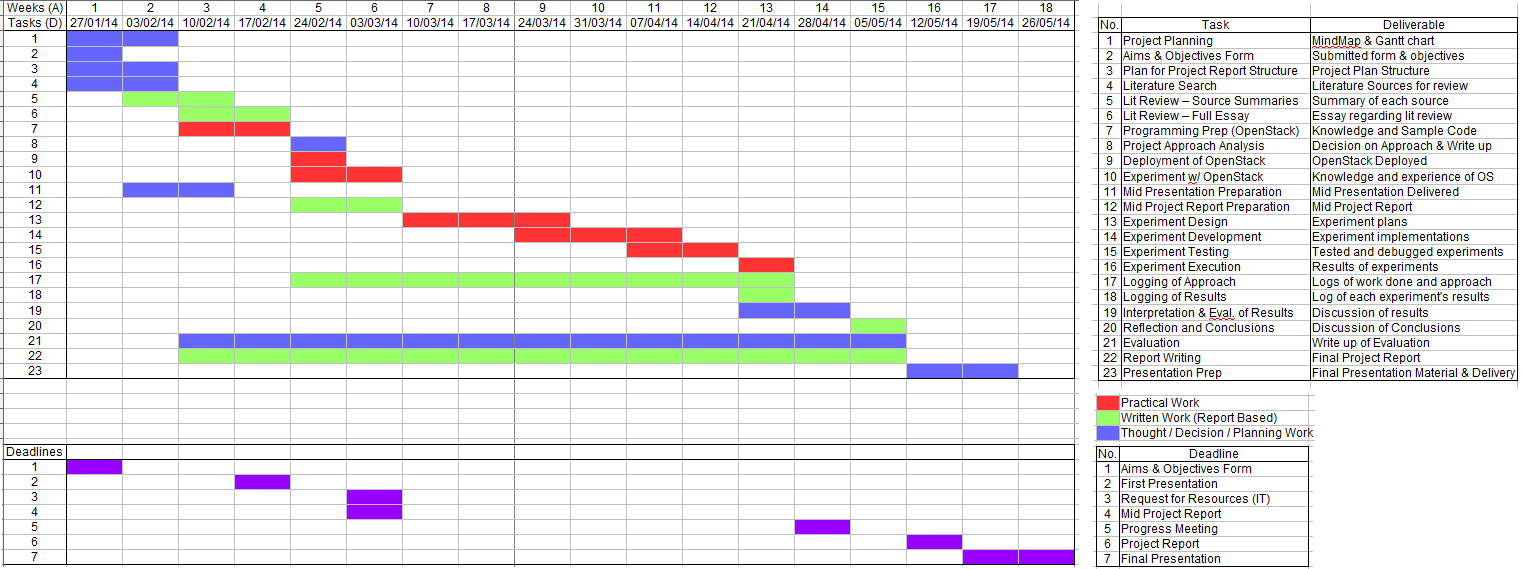
\includegraphics[scale=0.44]{joint-gantts3}}
\caption{GANTT Chart representing initial project schedule \& Deadlines}
\end{sidewaysfigure}



\begin{sidewaysfigure}
\centering
\fbox{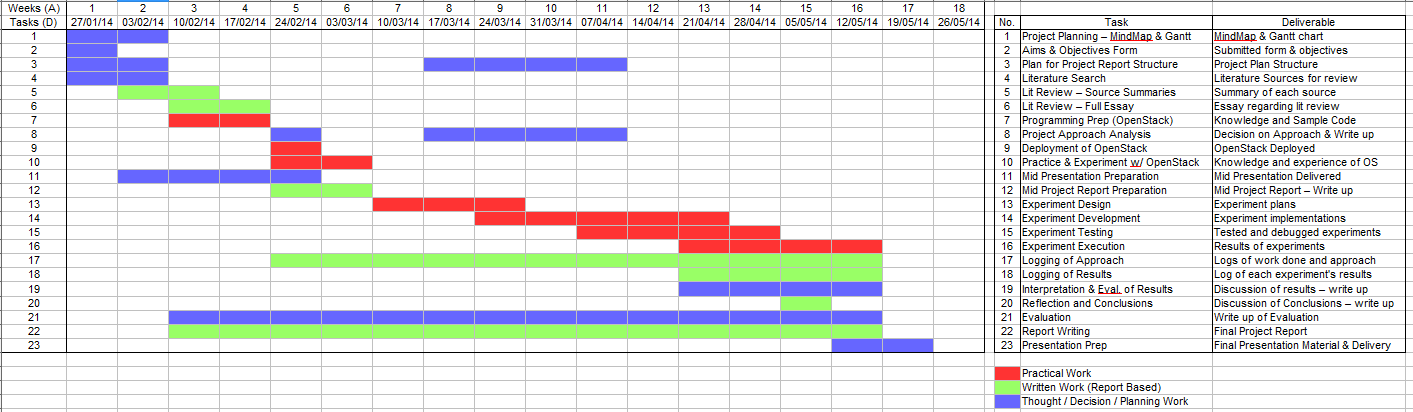
\includegraphics[scale=0.44]{final-gantt}}
\caption{GANTT Chart representing final project schedule}
\end{sidewaysfigure}
